\newpage
\section{Einleitung}
In diesem Dokument wird die Entwicklung der Applikation CharBuilder als Semesterprojekt für das Wahlpflichtfach Mobile Applikationen im fünften Semester dargestellt. Die Aufgabenstellung hat uns sowohl die Wahl der Plattform als auch die Art der App offengelassen. Da wir in der Vorlesung die Grundlagen der App-Entwicklung unter Android gelernt haben, machte es für uns Sinn, unsere erste App für Android zu entwickeln. Weitere Faktoren für die Entscheidung waren, dass man für die Entwicklung keinen teuren Development Account benötigt und beide Entwickler bereits Kenntnisse in Java besitzen. Außerdem kann die App direkt auf dem eigenen Smartphone getestet werden.\\

Die Idee der App entstand aus unserem gemeinsamen Hobby, dem Pen and Paper Rollenspiel. Pen and Paper Charaktere werden normalersweise am Computer generiert und verwaltet. Wenn man sich zum Spielen trifft, bringt jeder seinen Charakterbogen ausgedruckt oder als Datei auf dem Handy mit. Ziel der App ist es, sowohl neuen als auch erfahrenen Pen and Paper Spielern eine komfortable Lösung zu Erstellung und Verwaltung ihrer Charaktere auf dem Handy zu bieten. Dadurch kann man sich das Ausdrucken oder Übertragen aufs Handy sparen und man kann seine Charaktere überall mit hinnehmen.\\

Der Aufgabenstellung konnten wir die fünf Themengebiete Stand der Technik, Anforderungen, Architektur, Implementierung und Test und Usability für unsere Dokumentation entnehmen. Auf jedes dieser Themen werden wir im Verlauf der Dokumentation eingehen und dadurch strukturiert die Entwicklung der App aufzeigen.

\newpage
\section{Stand der Technik}
Im Nachfolgenden wird erläutert, welche Technologien wir für die Erstellung der CharBuilder App verwendeten und warum diese von uns gewählt wurden. Hierbei haben wir den Text in die Unterkategorien Android(Betriebssystem), Kotlin(Programmiersprache), Gson(Json Java-Lib), Gradle(Build Tool), Android Studio(IDEA), UMLet(UML Tool), Git und Google Firebase aufgeteilt. Das sind die wichtigsten Technologien, die wir zum Entwickeln unserer App genutzt haben.

\subsection{Android}
Wie in der Einleitung geschrieben, haben wir uns für Android als Betriebssystem entschieden. Da verschiedene Version dessen auf unterschiedlichen Geräten verteilt sind
muss man sich als Entwickler darüber hinaus auch für ein Mindest-API-Level entscheiden. Dies stellt die niedrigste Android Version dar, unter welcher die App ausgeführt werden kann.
Bei der Wahl des API-Levels spielen verschiedene Faktoren eine Rolle, unter anderem wie viele der Android Geräte welche Version des Betriebssystems ausführen oder ob der Entwickler
Funktionen nutzen möchte die erst ab einer bestimmten Version verfügbar sind.\\
%includegraphics("bild api verteilung android")
Wir haben uns entschieden, unsere Applikation lediglich für Android Betriebssysteme der Version 5.0(API Level 21) oder höher zu entwickeln.
Die Version 5 ist bereits am 12.11.2014 veröffentlicht worden und bringt einen großen Wandel in der Benutzeroberfläche durch Googles Material Design.
Dieses ist an den Gestaltungsstil "Flat Design" angelehnt und minimalistisch gehalten. Die Entscheidung trafen wir aufgrund der weitreichenden 
Änderungen in dieser Version, des bereits 3 Jahre in der Vergangenheit liegenden Veröffentlichungsdatums und der breiten Verteilung von 80,7\% aller Android Geräte.
%\cite{https://de.statista.com/statistik/daten/studie/180113/umfrage/anteil-der-verschiedenen-android-versionen-auf-geraeten-mit-android-os/}.\\

\subsection{Kotlin}

Kotlin ist eine neue Programmiersprache von JetBrains aus dem Jahr 2016. Wie auch Java kompiliert Kotlin zu JVM Bytecode. Es lässt sich dadurch sehr gut in das bestehende Java Ökosystem einbinden und kann alle Java Bibliotheken verwenden. Seit dem 17. Mai 2017 ist Kotlin eine von Android offiziel unterstützte Sprache.\cite{kotlinrelease}\\

Beide Teammitglieder haben zuvor noch nicht mit Kotlin gearbeitet, konnten sich jedoch aufgrund der Ähnlichkeit zu Java schnell zurechtfinden und gute Erfahrungen sammeln. Die Programmiersprache bietet dem Programmierer viele Vorteile wodurch sie immer beliebter wird unter Androidentwicklern. Der weitreichenste Vorteil ist es  null-Referenzen zu verhindern, die Sprache bietet einem "Null Safety". Eine weitere Änderung ist auch die Möglichkeit Datenklassen zu erstellen, diese sind Klassen welche lediglich Daten halten und keinerlei Methoden selbst implementieren. Ein Beispiel dieser kann man im Kapitel Implementierung finden. Der Großteil der Appentwicklung geschah mit Kotlin v1.15 später wurde dann ein Update auf Kotlin v1.2 durchgeführt. Dies liegt an dem Entwicklungszyklus von Kotlin, so wurde immer mit dem aktuellsten stabilen Release gearbeitet.\cite{kotlin}

\subsection{Gson}

Gson ist eine Java Bibliothek zur Serialization und Deserialization. Sie wird genutzt um Java Objekte in JSON umzuwandeln oder auch JSON zu Java Objekten zu wandeln. Hierbei ist die Möglichkeit Generics zu verwenden äußerst wichtig, da diese in der CharBuilder Applikation mehrmals zum Einsatz kommt. Wir haben diese Bibliothek ausgesucht da sie uns bereits bekannt war von früheren Projekten und wir positive Erfahrungen gemacht haben. Desweiteren wird die Software bereits seit 2008 entwickelt und konnte seitdem durch viele Revisionen und Verbesserungen überzeugen. Für die App verwendet wir die Gson Version 2.8.2.\cite{gson}

\subsection{Gradle}

Gradle ist ein weit verbreitetes Build-Tool, welches automatisiert arbeitet und Unterstützung für mehrere verschiedene Sprachen bietet. Es wird typischerweise für Android Applikationen verwendet, welche mit Android Studio entwickelt werden, da das Tool tief in die Entwicklungsumgebung integriert ist. Zu unserer Entscheidung dieses Programm zu verwenden kann nicht viel gesagt werden, da es wie oben erwähnt bereits integriert war und eine Alternative neben großem Mehraufwand keine Vorzüge geboten hätte.

\subsection{Android Studio}

Android Studio ist die offizielle Entwicklungsumgebung für native Androidprogrammierung. Es bietet neben den bekannten IDE Funktionen wie Syntax Highlighting, Autovervollständigung, Instant Run(Es wird nur der veränderte Teil neu kompiliert) und Debugger auch einen Android Emulator, um verschiede Geräte und Android Version zu simulieren. Die IDE basiert auf IntelliJ's Softwareprodukten. Mit der Version 3.0.1 wurde die Entwicklungsumgebung für Kotlin angepasst, dies ist auch die Version welche wir zur Entwicklung unserer App verwendeten. Dabei liefert die neue Version ebenfalls ein Programm, um Java-Code direkt in Kotlin-Code umzuwandeln.  Dem Entwickler wird so der Einstieg in Kotlin erleichtert, das Tool sollte im späteren Verlauf aber nur selten genutzt werden, um eine einheitliche Codequalität zu erreichen.

\subsection{Git}

Git ist eine Software zur Versionsverwaltung. Es findet bereits große Anwendung in der Industrie und ist neben SVN das bekannteste System. Hauptgrund für unsere Entscheidung Git zu nutzen war die bereits über die vergangene Semester gesammelte Erfahrung. Git bietet weiterhin den Vorteil das man getrennt arbeiten kann, da jeder eine lokale Arbeitskopie hat. Für unser Projekt verwendeten wir den Git-Serviceprovider Github, dieser stellt kostenloses ein Repository für uns zu Verfügung.

\subsection{UMLet}

UMLet ist ein kostenloses Open-Source UML Tool mit einer simplen Benutzeroberfläche. Die erstellten Diagramme lassen sich z.B. als pdf, jpg oder png exportieren. Wenn einem die große Auswahl an UML Elementen nicht reicht, kann man eigene erstellen oder importieren. Zum Zeichnen unserer Diagramme haben wir die Version 14.2 genutzt.\cite{umlet}

\subsection{Google Firebase}
\label{sdt:firebase}

Firebase ist eine Entwicklungsplattform für Mobile- und auch Webapplikationen. Ursprünglich als Startup 2011 gegründet wurde es 2014 von Google aufgekauft. Der Dienst bietet mehrere Funktionen, in unserer App verwenden wir allerdings nur \textit{Firebase Storage} verwendet um dem Nutzer das speichern seines Charakters zu ermöglichen. Hier bietet der Service eine Stufe welche es uns ermöglicht die Anwendung im kleinen Rahmen zu verwenden ohne das zusätzliche Kosten entstehen.

\newpage
\section{Anforderungen}
Im folgenden Kapitel werden die Anforderungen, die wir an unsere App gestellt haben, genauer beschrieben. Diese Anforderungen wurden von uns vor Beginn der App-Implementierung aufgestellt, um einen Überblick über alle Funktionen zu erhalten, die die App beinhalten wird. Die Anforderungen sind in diese vier Kategorien eingeteilt:
\begin{description}
\item[Must Have]\hfill \\
Unter \grqq Must have\grqq{} ist jede Funktionalität aufgelistet welche \textbf{unbedingt} umgesetzt werden muss, um das Projekt als erfolgreich bezeichnen zu können. Diese Kategorie wird oft auch \grqq Minimale Anforderungen\grqq{} genannt.
\item[Should Have]\hfill \\
Die Kategorie \grqq Should have\grqq{} fasst all die Punkte unter sich zusammen, die für ein erfolgreiches Projekt nicht unbedingt erforderlich sind, aber dennoch wichtiger Bestandteil sein können. Als Beispiel sei eine Funktionalität zu sehen, welche das Produkt lediglich erweitert, von welcher die Grundfunktionalitäten allerdings nicht abhängig sind.
\item [Could Have]\hfill \\
Features, die unter \grqq Could have\grqq{} aufgelistet sind, werden nur umgesetzt, wenn alle Punkte unter \grqq Must have\grqq{} und \grqq Should have\grqq{} bereits abgearbeitet sind. Sie sind vollkommen optional.
\item[Won't Have]\hfill \\
\grqq Won't have\grqq{} beinhaltet jene Punkte, welche \textbf{nicht} umgesetzt werden. Sie wurden von den Entwicklern oder Auftraggebern zu Beginn der Projektspezifikation ausgeschlossen.
\end{description}

\subsection{Must Have}
Als wichtigste Funktion der App gilt das Erstellen eines neuen Charakters. Es muss möglich sein einen Charakter entsprechend des gewählten Regelwerks zu erstellen. Zunächst wird es nur möglich sein Charaktere im Regelwerk \textit{Star Wars: Am Rande des Imperiums} zu erschaffen. Während des Erstellungsprozesses kann der Nutzer auf Regeltexte zurückgreifen, die ihm seine aktuellen Auswahlmöglichkeiten erklären. Diese Regeltexte werden aufgrund von eventuellen Urheberrechtsverletzungen nicht aus dem offiziellen Regelwerk kopiert, sondern von den Entwicklern der App zusammengefasst.\\

Nachdem der Nutzer einen Charakter erstellt hat, wird dieser in einer Liste mit anderen bereits von ihm angelegten Charakteren angezeigt. In der Liste wird das für den Charakter ausgewählte Bild, sein Name und das Regelwerk, in dem er gespielt wird, dargestellt. Der Nutzer kann nicht mehr benötigte Einträge aus der Liste löschen, Änderungen an den Charakteren vornehmen und diese als PDF-Datei exportieren. Durch einen Klick auf einen der Listeneinträge werden dem Nutzer alle Eigenschaften, Talente, Spezialisierungen, etc. zu einem Charakter angezeigt.\\

Eine weitere Funktion der App ist das eingebaute Würfeltool. Wenn der Nutzer sich in der Detailansicht zu einem seiner Charaktere befindet, kann er ohne großen Aufwand Proben auf seine Fähigkeiten werfen. Es wird dann berechnet, ob die Probe erfolgreich war oder nicht und das Ergebnis erscheint in einem Dialog. Außerdem wird das Ergebnis des Würfelwurfs im Verlauf des Würfeltools angezeigt, sodass der Nutzer eine Übersicht seiner vorherigen Proben erhält. Das Würfeltool ist über die Navigationsleiste im Hauptmenü erreichbar und bietet eine Auswahl an Würfeln, die für das jeweilige Regelwerk benötigt werden.

\subsection{Should Have}
Damit Charaktere nicht an ein bestimmtes Gerät gebunden sind, sollte der Nutzer die Möglichkeit haben, seine Charakterdaten als JSON-Datei in Google Drive zu speichern. Jeder Charakter bereist im Zuge seiner erlebten Abenteuer eine Vielzahl von Orten. Um dem Spieler eine Erinnerungsstütze zu geben, an welchen Orten sein Charakter schon war und was für Abenteuer er dabei abgeschlossen hat, sollte es eine Art Reisetagebuch für jeden Charakter geben.

\subsection{Could Have}
Es wird nicht ausgeschlossen, dass die App die Erstellung von Charakteren in unterschiedlichen Regelwerken ermöglicht. Allerdings gibt es große Unterschiede in der Komplexität und dem Umfang von Pen and Paper Regelwerken, weswegen zunächst nur ein Regelwerk unterstützt wird. Eine englischsprachige Version der App ist geplant. Das Übersetzen der Regeln nimmt jedoch viel Zeit in Anspruch. Eine weitere mögliche Option wäre das Einbinden der Google Billing API, die dem Entwickler das Freischalten von In-App Käufen ermöglicht.

\subsection{Won't Have}
Die App wird keine Gruppenverwaltung ermöglichen. Das bedeutet, dass ein Spielleiter nicht die Charaktere seiner Gruppenmitglieder einsehen kann. Außerdem werden in der App keine spielbaren Abenteuer vorhanden sein. Sie dient lediglich dem Speichern und Verwalten von Pen and Paper Charakteren. Nutzer der App werden in der App keine Anleitung für das Spielen von Pen and Paper Abenteuern finden. Alle verwendeten Auszüge aus Regelwerken dienen ausschließlich der Unterstützung während des Erstellungsprozesses. 

\newpage
\section{Architektur}
Dieses Kapitel beschäftigt sich mit der Architektur unserer App. Dazu werden wir zunächst den Aufbau der Packages und die Beziehungen der einzelnen Klassen untereinander anhand des Klassendiagramms darstellen, bevor wir näher auf das Model View Controller Pattern eingehen.

\subsection{Klassendiagramm}
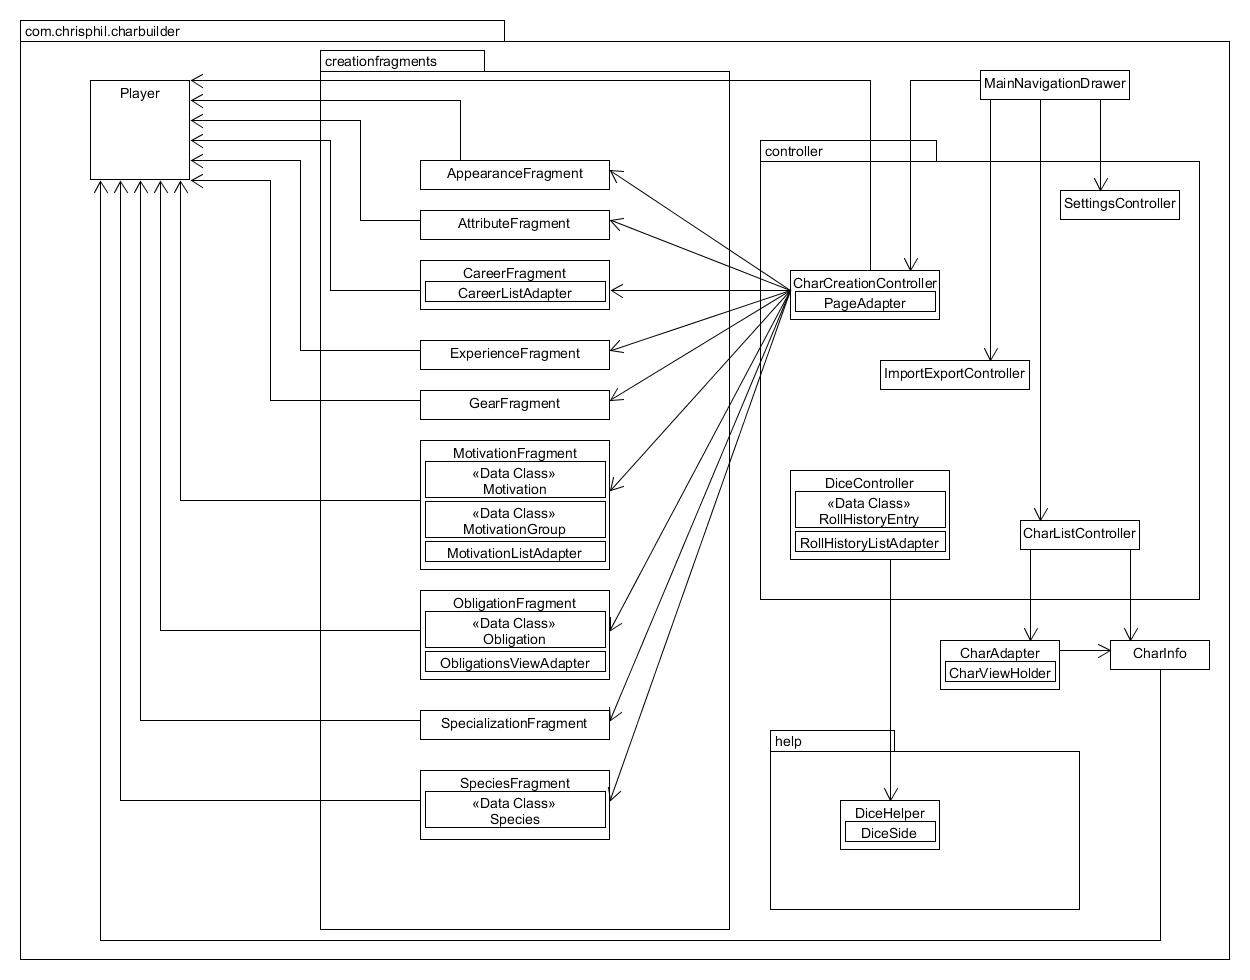
\includegraphics[scale=0.35]{images/klassendiagramm.jpg}

Das oben zusehende Klassendiagramm zeigt alle für die Applikation gebrauchten Klassen und die Pakete, in die sie eingeteilt sind. In den nächsten Absätzen werden die einzelnen Pakete und ihre zugehörigen Klassen bescreiben.

\subsubsection{com.chrisphil.charbuilder}
Eine Einordnung in eindeutige Pakete ist nicht für jede Klasse möglich. Aus diesem Grund werden solche Klassen in diesem Paket zusammengefasst.\\

Der \textit{MainNavigationDrawer} ist eine dieser Klassen. Als Mainactivity der App können von ihm die Klassen \textit{CharListController}, \textit{DiceController}, \textit{SettingsController} und \textit{ImportExportController} aufgerufen werden.\\

Als meistgenutzte Klasse hat \textit{Player} die meisten Verbindungen zu anderen Klassen. Das Laden und Speichern der Charakterdaten wird in dieser Klasse umgesetzt. Außerdem werden Daten aus den \grqq CreationFragments\grqq{} in einer Instanz der \textit{Player}-Klasse während der Charaktererstellung zwischengespeichert. 

Die letzten beiden Klassen dieses Pakets sind der \textit{CharAdapter} und die \textit{CharInfo}. Der \textit{CharAdapter} dient als Adapter, der für die Charakterliste des \textit{CharListControllers} eingesetzt wird. Den Inhalt dieser Liste bildet die \textit{CharInfo}, welche die geladenen Daten aus der \textit{Player}-Klasse mit den zugehörigen Bildern der Charaktere verbindet und an den \textit{CharAdapter} weitergibt.

\subsubsection{com.chrisphil.charbuilder.controller}
Unsere ursprüngliche Architektur sah vor, dass jedes Fragment, das durch den Nutzer über den \textit{MainNavigationDrawer} erreicht werden kann, einen eigenen Controller besitzen wird. Auf diese Weise sollten Darstellung und Datenverarbeitung getrennt werden. Alle benötigten Controller werden in diesem Paket gebündelt. Da diese Architektur sich als unpraktisch erwiesen hat, wurden alle mit dem \textit{MainNavigationDrawer} verbundenen Klassen zu eigenständigen Fragmenten ohne zugehörigen Controller.\\

Die einzige Klasse, welche ihre Funktion als Controller mehr oder weniger behalten hat, ist der \textit{CharCreationController}. Sämtliche Navigation der Charaktererstellung wird durch diese Activity geleitet, weshalb sie eine Verbindung zu jedem der \grqq CreationFragments\grqq{} besitzt. Außerdem wird in ihr eine Instanz der \textit{Player}-Klasse erzeugt.

\subsubsection{com.chrisphil.charbuilder.creationfragments}
Jedes der Fragmente in diesem Paket wird während der Charaktererstellung benötigt. Einige verfügen über innere Adapter-Klassen zum Füllen von Listen. Fragmente mit \grqq Data Classes\grqq{} lesen Daten aus XML-Dateien ein. Die Daten der Fragmente werden während der Charaktererstellung in einem Objekt der \textit{Player}-Klasse zwischengespeichert, welche zur \textit{CharCreationController}-Activity gehört.

\subsubsection{com.chrisphil.charbuilder.help}
Das Paket \grqq Help\grqq{} wurde erstellt, um Klassen zu sammeln, die eventuell mehrfach genutzte Programmlogik enthalten. So kann der Code aus dem \textit{DiceHelper} z.B. nicht nur im \textit{DiceController} angewendet werden, sondern bei Bedarf auch aus anderen Klassen heraus aufgerufen werden.

\subsection{Model View Controller(MVC)}
Model View Controller\cite{mvc} ist ein bekanntest Software Architektur \textit{Pattern}. In diesem wird der Quellcode in die 3 Bereiche Model(Datenrepräsentation), View(Darstellung) und Controller(Programmlogik) aufgeteilt. Das dient der Wiederverwendbarkeit von Code und unterstützt durch Kapselung die parallele Programmierung.
\newline Das Anwenden des MVC-Patterns ist nicht unüblich bei Android Applikationen, so entschieden wir uns auch dafür. Ursprünglich war geplant das die jeweiligen Controllerklassen (\textit{CharCreationController}, \textit{DiceController} usw.) die Programmlogik darstellen und neben den Views(Layoutdateien) die Playerklasse das Model repräsentiert. Dies lies sich aufgrund der vielen Fragmente bei der Charaktererstellung nur bedingt einhalten, das parallele Programmieren wurde durch diese Struktur dennoch unterstützt.
\newline Die Klasse \textit{Player} welche wie erwähnt als Model dient wurde von uns ebenfalls entwickelt damit alle Fragmente zu jeder Zeit die aktuellen Daten einsehen und so auf Veränderungen reagieren können. Insgesamt hatte das \textit{Pattern} einen positiven Einfluss auf unsere Softwarearchitektur. Um MVC umzusetzen mussten wir uns im Vorfeld bereits mit Struktur, Datenkapselung und Modellen beschäftigen, so dass von beginn an der Aufbau der Applikation festgelegt war.\\
\begin{figure}
	\centering
	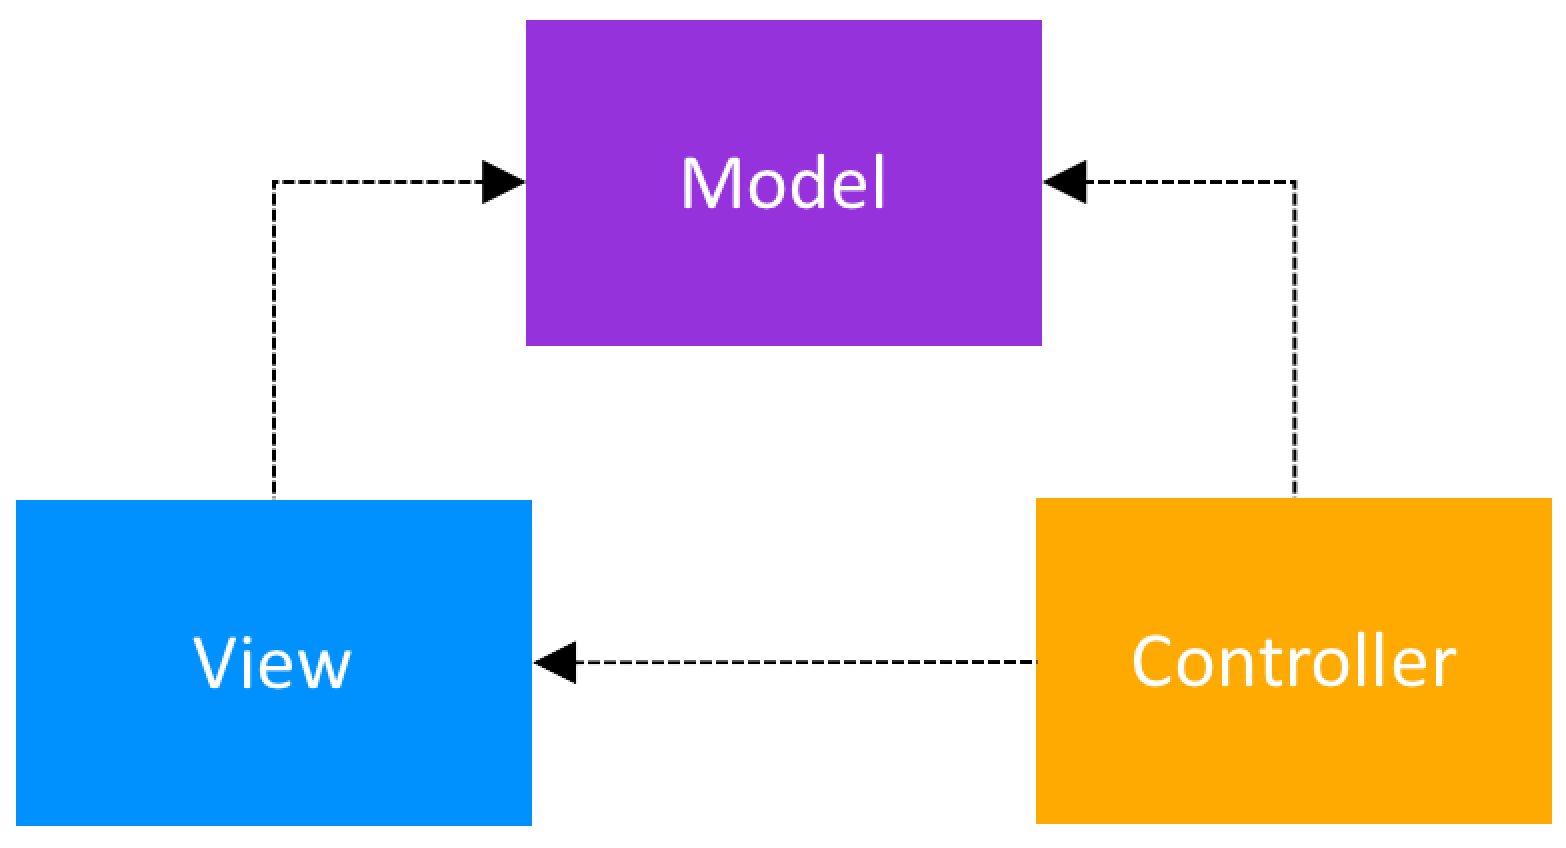
\includegraphics[width=0.5\textwidth]{images/mvc.png}
	\caption{Das Model View Controller Pattern}
\end{figure}

\newpage
\section{Implementierung}

\subsection{Charaktererstellung}
Da die Erstellung eines Charakters im offiziellen Regelwerk bereits in sinnvolle Schritte unterteilt war, wollten wir diese Gliederung in der App wiederspiegeln. Durch das Bewahren der in den Regeln eingeführten Struktur haben neue Spieler einen guten Überblick über die für die Charaktererstellung benötigten Schritte. Außerdem müssen sich Spieler, die das offizielle Regelwerk bereits kennen, nicht an eine neue Gliederung gewöhnen. In der App werden die Schritte durch Fragmente dargestellt. Jedes Fragment besitzt ein eigenes Layout, das an die Anforderungen des jeweiligen Erstellungsschritts angepasst ist. Für die Navigation zwischen den einzelnen Fragmenten verwenden wir ein \textit{TabLayout}. Dieses Layout wird durch die Klasse \textit{CharCreationController} mit den nötigen Tabs versehen.\\

Der \textit{CharCreationController} ist eine Activity, die geöffnet wird, sobald der Nutzer die Charaktererstellung startet. Er besitzt eine innere Klasse namens \textit{PageAdapter}, welcher von der durch Android zu Verfügung gestellten Klasse \textit{FragmentStatePagerAdapter} erbt. Durch den \textit{PageAdapter} wird geregelt, wann ein neues Fragment geladen wird und an welcher Stelle des \textit{TabLayouts} dieses Fragment eingeordnet wird. Das \textit{TabLayout} bietet dem Nutzer eine gute Übersicht über die Schritte der Charaktererstellung. Durch Klicken auf die Namen der einzelnen Tabs oder das Wischen nach links oder rechts kann der Nutzer frei wählen, welche Schritte des Erstellungsprozesses er bearbeiten möchte. Zudem kann er nachträglich Änderungen an Fragmenten vornehmen, falls ihm seine derzeitige Wahl nicht gefällt.\\

Jede Eingabe, die der Nutzer während der Erstellung in den Fragmenten einträgt, wird an die Activity weitergegeben, welche die Daten in einer Instanz der Klasse \textit{Player} speichert. Bei Initialisierung eines neuen Fragments wird geprüft, ob schon Werte in den entsprechenden Attributen des Player-Objekts vorhanden sind. Hat der Nutzer das geladene Fragment schonmal bearbeitet und möchte jetzt Änderungen vornehmen, sollen die Felder wieder so ausgefüllt sein, wie er sie hinterlassen hat. Eine weitere potenzielle Quelle für Verlust von Daten ist das versehentliche Drücken der Zurück-Taste auf der \textit{Android Navigation Bar}. Zur Vermeidung dieses Problems fängt die Activity Klicks auf die Zurück-Taste ab und zeigt einen Dialog an, in dem man das Abbrechen der Charaktererstellung bestätigen muss.\\

Es gibt zwei Layouts, die in mehreren Fragmenten als Listenelement in \textit{ListViews} oder als Group Item in \textit{ExpandableListViews} eingesetzt werden:
\begin{description}
\item[char\_creation\_listview.xml]\mbox{}\\
Ein Layout bestehend aus zwei \textit{TextViews} für Name und kurz Beschreibung des jeweiligen Elements und einem anklickbaren \textit{ImageView}, das, wenn der Nutzer darauf drückt, einen Dialog mit dem Regeltext zum jeweiligen Element wiedergibt.
\item[char\_creation\_career\_group\_item.xml]\mbox{}\\
Dieses Layout besteht nur aus einem \textit{TextView} und wird in \textit{ExpandableListViews} als Group Item Layout verwendet.
\end{description}

Einige der Fragmente verfügen über eine \textit{Data Class}. Diese Klassen sind ein in Kotlin eingeführtes Konzept, um das Schreiben von unnötigem \grqq Boilerplate Code\grqq{} in einfachen Klassen, die nur als Datencontainer genutzt werden, zu verhindern \cite{dataclasses}. Häufig werden die Datenklassen in den Fragmenten dazu genutzt, Daten aus einer geparsten XML-Datei zu speichern und sie dann in ein \textit{ListView}-Element zu laden. Mit Hilfe dieser Methode erleichtern wir uns das Zuordnen der passenden Kurzbeschreibungen und Regeltexte zu einem entsprechenden Regelbegriff.\\

Im Folgenden werden wir auf die einzelnen Fragmente und ihre Funktionen eingehen. Sie sind in der Reihenfolge angeordnet, in der sie auch in den Tabs der Charaktererstellung  wiederzufinden sind.

\subsubsection{ObligationFragment.kt}
Der erste Schritt in einer Charaktererstellung ist das Bestimmen der Verpflichtung/en eines Charakters. Das Regelwerk zu \glqq Star Wars : Am Rande des Imperiums\grqq{} \cite[39]{rulebook} gibt eine Liste von zwölf wählbaren Pflichten vor. Dem Spieler werden zwei Möglichkeiten angeboten, eine Pflicht für seinen Charakter zu wählen:
\begin{enumerate}
\item Der Spieler sucht sich aus der Liste mit zwölf Einträgen eine für ihn passende Pflicht aus.
\item Durch das Drücken auf einen Button lässt der Spieler die App per Zufall ein oder zwei Pflichten bestimmen.
\end{enumerate}

Zur Umsetzung der Liste haben wir uns für eine \textit{ListView} entschieden, die durch die innere Klasse \textit{ObligationsViewAdapter} mit Inhalt gefüllt wird. Der \textit{ObligationsViewAdapter} ist eine Unterklasse des \textit{BaseAdapters} aus der Android API, welcher in der \textit{onCreateView}-Methode des Fragments als Adapter der \textit{ListView} gesetzt wird. Mit der Liste aus Pflichten, die zuvor aus einer XML-Datei geparst wurde, erstellt der Adapter dann jedes Listenelement anhand des Layouts aus der \textit{char\_creation\_listview.xml}. Nachdem ein Listenelement angeklickt wurde, wird es blau hinterlegt und der Name der Pflicht wird als aktuell ausgewählte Pflicht im oberen Textfeld angezeigt.\\

Jede Pflicht hat eine Wahrscheinlichkeit von 8\% durch den Zufall ausgewählt zu werden. Insgesamt hat der Spieler also eine Chance von 96\% nur eine Pflicht bei der zufälligen Bestimmung zu erhalten. Die übrigen 4\% bilden die Wahrscheinlichkeit dafür, dass der Charakter mit zwei Pflichten startet. Diese Warscheinlichkeiten für das Auswählen der Pflichten wurden dem Regelwerk \cite[39]{rulebook} entnommen, das eine Tabelle mit Würfelergebnissen für jede Verpflichtung beinhaltet. Während der Erstellung ist die Zufallsbestimmung der einzige Weg, eine zweite Verpflichtung zu erhalten. Aus diesem Grund musste in der Implementierung darauf geachtet werden, dass das Textfeld der zweiten Pflicht zurückgesetzt wird, wenn eine neue ausgewählt wird. Dabei ist es egal, ob die neue Verpflichtung durch den Spieler oder den Zufall gesetzt wird. Wenn die derzeitige Pflicht dem Spieler nicht gefällt, kann er sie beliebig oft selbst ändern oder durch Drücken des Buttons neu bestimmen. Die Reihenfolge der Aktionen spielt dabei keine Rolle.\\

\subsubsection{SpeciesFragment.kt}

Das SpeciesFragment bietet dem Nutzer eine Liste an, aus welcher ein Element ausgewählt werden muss. Zusätzlich bietet jedes Listenelement eine weitere Schaltfläche an, welche ein Dialogfenster mit zusätzlichen Informationen öffnet. Zu Beginn der Implementierung haben wir uns überlegt wie man die einzelnen Spezies gut darstellen kann ohne den Anwender mit den vielen Informationen zu überfordern. Hier entschieden wir uns dann für die oben genannte Liste, welche jeweils den Namen und eine beschreibenden Satz zu jeder Spezies anzeigt. Sollte der Benutzer sich dann noch weitere Informationen anzeigen lassen wollen so kann er das mit der auf der linken Seite dargestellten Schaltfläche tun. Intern wird jedes Element durch die Klasse \textit{Species} repräsentiert. Diese enthält insgesamt 13 Variablen um jede Eigenschaft gut darstellen zu können. Ein wichtiger Punkt war für uns das speichern der Daten. Hier entschieden wir uns für eine XML-Datei, da Android bereits Funktionen zum Laden und Manipulieren dieser bietet. Wir legten also zusätzlich zum \textit{SpeciesFragment} und der entsprechenden Layout-Datei auch eine \textit{Species.xml} an in welche wir die statischen Daten eingetragen haben. Diese wird dann mittels des \textit{XMLPullParser}'s eingelesen und die entsprechenden Spezies Objekte erstellt. Das Layout des Fragmentes ist entsprechend simpel aufgebaut und enthält lediglich eine \textit{ListView}. Mittels der von uns angelegten Klasse \textit{SpeciesViewAdapter} konnten wir den Inhalt der Listenelemente dann entsprechend setzen. Zuletzt erstellten wir dann eine Methode \textit{createSpeciesInfoDialog} welche ein Spezies Objekt erwartet und aus diesem dann einen entsprechenden Dialog erzeugt welcher mehr Informationen darstellt, da in der Liste lediglich Name und Beschreibung angezeigt werden. Die Liste befindet sich im sogenannten \textit{SINGLE\_CHOICE\_MODE} damit der Nutzer wirklich nur ein Element auswählen kann, dieses wird dann farblich hervorgehoben. Zu diesem Fragment lässt sich abschließend sagen, dass die Implementierung beim ersten Ansatz gut umgesetzt werden konnte. Dies liegt unter anderem an dem einfachen Aufbau und der guten XML-Datei Unterstützung der Android API.

\subsubsection{CareerFragment.kt}

Das CareerFragment biete eine ähnliche Funktionalität wie das oben genannten SpeciesFragment, es ist jedoch aufgrund der gesteigerten Komplexität nicht so unkompliziert zu implementieren. Wegen der größeren Menge an Daten und Abhängigkeiten, welche dargestellt werden müssen, haben wir uns entschieden als Hauptelement der Benutzeroberfläche eine \textit{ExpandableListView} zu verwenden. Sie besteht aus \textit{GROUP\_ITEM}'s welche jeweils beliebig viele \textit{CHILD\_ITEM} haben können. Diese \textit{CHILD\_ITEM}'s werden bei der Auswahl des Gruppenelements \grqq ausgeklappt\grqq{}. Auf diese weise ist es möglich die Abhängigkeiten für den Nutzer gut sichtbar zu modellieren. Sollte der Anwender dann eines der Subelemente auswählen, öffnet sich der entsprechende \textit{Skill Tree} und die Applikation merkt sich welcher Beruf ausgewählt wurde. Da die Daten dieses Fragmentes an die Auswahl der Spezies gebunden ist, wird der Nutzer bei Änderungen oder Inkonsistenzen mittels eines Dialoges benachrichtigt. Durch die vielen Elemente mussten bereits nur für die Liste drei Layout-Dateien angelegt werden. In der \textit{char\_creation\_career.xml} wird lediglich die \textit{ExpandableListView} angelegt, die anderen beiden Dateien sind jeweils für das Gruppen- und Kindelement: \textit{char\_creation\_career\_group\_item.xml} und \textit{char\_creation\_career\_child\_item.xml}. Im eigentlichen Quellcode ähnelt dieses Fragment sehr dem oben genannten, ein möglicher Beruf wird um Beispiel durch die Klasse Career repräsentiert. Sie bietet unter anderem die Variablen für Namen und die entsprechenden Unterklassen welche die Kindelemente darstellen. Die Daten werden wieder mit dem  \textit{XMLPullParser} eingelesen, womit dann die Objekte erstellt werden. Die Daten zu den \textit{Skill Tree}'s werden ebenfalls aus einer XML-Datei geladen. Sollte der Nutzer seine bisherige Auswahl ändern wollen so kann er dies mit einem einfachen Button tun.

\subsubsection{SpecializationFragment.kt}

Als wir anfangs den Aufbau unserer App geplant haben wurde festgelegt das jeder Schritt des Regelwerks als ein Fragment der Charaktererstellung umgesetzt wird. Als wir allerdings das \textit{CareerFragment} implementiert haben, wurden wir auf die enge Verzahnung der beiden Schritte aufmerksam. Aufgrund dieser Erkenntnisse entschieden wir, dieses Fragment komplett von dem Inhalt des \textit{CareerFragment}'s abhängig zu machen. Sobald sich die Daten in diesem ändern, wird das \textit{SpecializationFragment} zurückgesetzt. So kann gewährleistet werden das der Nutzer keine Eingaben tätigt welche sich gegenseitig widersprechen.

\subsubsection{ExperienceFragment.kt}
Nachdem der Spieler sich im vorherigen Fragment eine Spezialisierung seines Berufs ausgesucht hat, kann er hier Erfahrungspunkte einsetzen, um bestimmte Fähigkeiten zu erlernen. Dazu wird ihm der Talentbaum seiner Spezialisierung und die einsetzbaren Erfahrungspunkte angezeigt. Wie viele Erfahrungspunkte dem Spieler zum Erlernen neuer Fähigkeiten zur Verfügung stehen, hängt von der zuvor gewählten Spezies ab. Das bedeutet, das beim Öffnen des Fragments einige Voraussetzungen geprüft werden müssen. Sind diese Bedingungen nicht erfüllt, wird dem Nutzer ein Dialog angezeigt, in welchem er über die Änderungen im Fragment informiert wird.\\

Ein möglicher Auslöser für einen solchen Dialog ist das Wechseln der Spezies durch den Spieler. Wird dem Charakter eine neue Spezies zugewiesen, ändert sich dadurch die Menge an Erfahrungspunkten, die der Spieler im \textit{ExperienceFragment} ausgeben kann. Da der Spieler durch die Änderung der Spezies eventuell nicht mehr genügend Erfahrungspunkte hat, um zuvor erlernte Fähigkeiten weiterhin freischalten zu können, muss das Fragment bei einem Wechsel der Spezies zurückgesetzt werden. Ein Zurücksetzen des Fragments wird auch durch die Neuwahl des Berufs oder der Spezialisierung ausgelöst. Ein anderer Beruf sorgt dafür, dass dem Spieler andere Spezialisierungen zur Auswahl stehen. Durch eine neue Spezialisierung können mit den Erfahrungspunkten andere Fähigkeiten als zuvor freigeschaltet werden. Sollte der Nutzer das \textit{ExperienceFragment} aufrufen, ohne eine Spezies, einen Beruf oder eine Spezialisierung festgelegt zu haben, kann er das Fragment nicht nutzen, weil die fehlenden Informationen notwendig für das Verteilen der Erfahrungspunkte und Erlernen von Fähigkeiten benötigt werden. Wenn dieser Fall eintritt, wird ein Dialog geöffnet, der dem Nutzer alle Fragmente auflistet, welche er noch anschließen muss, bevor er das \textit{ExperienceFragment} bearbeiten kann.

\subsubsection{AttributeFragment.kt}

Das \textit{AttributeFragment} ist lediglich da um dem Spieler seine Attribute anzuzeigen. Dies ist nötig da sie teilweise aus den bereits eingetragenen Daten berechnet werden und der Nutzer sonst keine Möglichkeit diese abzufragen. Dieses Fragment ist aus einer anfänglichen Fehleinschätzung entstanden, da entgegen unserer annahmen der Spieler keinen direkten Einfluss auf die Attribute hat. Dieses Fragment besitzt ebenfalls eine Layoutdatei \textit{char\_creation\_attribute.xml} um das aussehen zu beschreiben.

\subsubsection{MotivationFragment.kt}
In diesem Schritt der Charaktererstellung wählt der Spieler die Motivation des Charakters aus. Es gibt insgesamt 30 Motivationen, die in drei Oberkategorien mit jeweils zehn Motivationen eingeteilt sind. Wie auch im \textit{ObligationFragment} hat der Spieler zwei Möglichkeiten zur Auswahl:
\begin{enumerate}
\item Der Spieler sucht sich aus den drei Oberkategorien mit insgesamt 30 Einträgen eine für ihn passende Motivation aus.
\item Die App bestimmt durch Drücken eines Buttons per Zufall ein oder zwei Motivationen.
\end{enumerate}

Zur Umsetzung der Listen mit den drei Oberkategorien nutzen wir eine \textit{ExpandableListView}, da sie genau die Eigenschaften mitbringt, die für so eine Darstellung nötig sind. Wenn der Nutzer zu diesem Fragment wechselt, sieht er zunächst nur die drei Oberkategorien Zielsetzung, Beweggrund und Bindung. Diese Group Items besitzen das Layout der \textit{char\_creation\_career\_group\_item.xml}, welches ihnen durch den \textit{MotivationListAdapter} zugeteilt wird. Als Unterklasse des \textit{BaseExpandableListAdapters} wird der \textit{MotivationListAdapater} in der \textit{onCreateView}-Methode des Fragments als Adapter der \textit{ExpandableListView} eingesetzt. Klickt der Nutzer auf ein Group Item, wird die Liste mit den zugehörigen Motivationen entfaltet. Das Layout der Child Items ist wiedermal die \textit{char\_creation\_listview.xml}.\\

Da die Motivationen in drei Kategorien eingeteilt sind, verlief die Bestimmung der Motivationen per Zufall etwas anders als im \textit{ObligationFragment}. Zunächst wurden anhand einer Tabelle im Regelwerk \cite[94]{rulebook} die Wahrscheinlichkeiten der Oberkategorien entnommen. Die Tabelle gibt für jede der Kategorien eine Wahrscheinlichkeit von 30\% an. Die übrigen 10\% geben die Chance wieder, bei der Erstellung eine zweite Motivation zu bekommen. Tritt dieser Fall ein, müssen zwei Kategorien ausgewürfelt werden. Nachdem eine oder zwei Kategorien bestimmt wurden, aus denen eine Motivation gewählt wird, erfolgt ein erneuter Zufallswurf. Für diese Zufallsbestimmung liegt die Wahrscheinlichkeit für alle Motivationen der jeweiligen Gruppe bei 10\%. Auch in diesem Fragment gilt die Zufallsbestimmung als einzige Möglichkeit, eine zweite Motivation zu erhalten. Beim Klicken auf ein Child Item oder das erneute Drücken des Zufallsbuttons wird das Feld für die zweite Motivation zurückgesetzt.\\

Die \textit{ExpandableListView} war nicht unsere erste Wahl zur Darstellung der Motivationen. Das ursprüngliche Layout des Fragments bestand aus drei untereinander angeordneten \textit{ListViews}, welche
durch \textit{TextViews} mit den Namen der jeweiligen Gruppen voneinander abgegrenzt werden sollten. Damit der Nutzer alle drei \textit{ListViews} durch Scrollen erreichen kann, sollten sie in einer \textit{ScrollView} angeordnet sein. Android lässt es allerdings nicht zu, zwei scrollbare Elemente ineinander zu verschachteln. Also musste die einfache Lösung, die bereits im \textit{ObligationFragment} Verwendung gefunden hat, einer komplexeren Lösung weichen. Unser nächster Ansatz war, die drei \textit{ListViews} in \textit{CardViews} zu verpacken und diese dann untereinander anzuorden. Diese Lösung war auch nicht optimal, da die \textit{ListViews} dann auf eine minimal Größe zusammengeschrumpft sind, sodass der Nutzer keine gute Ansicht der Motivationen hatte. Schließlich wurde die Idee der drei \textit{ListViews} komplett verworfen. Der frühere \textit{BaseAdapter} musste durch einen mit wesentlich höherem Implementierungsaufwand verbundenem \textit{BaseExpandableListAdapter} ersetzt werden und die drei \textit{ListViews} wurden in einer \textit{ExpandableListView} zusammengefasst.

\subsubsection{AppearanceFragment.kt}
Für das Layout dieses Fragments wurde mehr Zeit in Ansrpuch genommen als ursprünglich eingeplant. Zuerst sollten sich alle Elemente in einem \textit{RelativeLayout} befinden und durch mögliche Abhängigkeiten wie \textit{android:layout\_below} an ihre angedachte Position geschoben werden. Mit diesem Aufbau des Layouts wurden die \textit{TextViews} jedoch nicht auf einer Linie mit den \textit{EditText}-Elementen gezeichnet, so dass immer ein Höhenunterschied sichtbar war. Der zweite Ansatz bestand aus zwei \textit{LinearLayouts}, die mit Hilfe eines \textit{RelativeLayouts} parallel nebeneinander angeordnet werden und dafür sorgen, dass jeweils ein \textit{EditText}-Element auf der selben Höhe wie das zugehörige \textit{TextView} platziert wird. Das Ergebnis war das selbe wie zuvor. Der dritte Entwurf brachte endlich das erhoffte Ergebnis. Als Root-Layout wird wieder ein \textit{RelativeLayout} genutzt, um die schon erwähnten Abhängigkeiten nutzen zu können. Danach verwenden wir für jedes Paar aus \textit{TextView} und \textit{EditText} ein eigenes \textit{LinearLayout} mit einer horizontalen Ausrichtung. Nur das letzte Paar ist vertikal angeordnet, da die Eingabe im \textit{EditText} eventuell länger werden könnte.\\

Zusammen mit dem \textit{GearFragment}, das im nächsten Absatz beschrieben wird, ist das \textit{AppearcanceFragment} das einzige Fragment, in dem der Spieler eigene Texteingaben vornehmen kann. Je nachdem, welche Eingabe der Nutzer im jeweiligen \textit{EditText}-Element eintragen soll, wird ihm eine passende Tastatur angezeigt. Verlangt das Eingabefeld z.B. ein Alter für den Charakter, so wird dem Nutzer nur eine Tastatur mit Zahlen als Eingabeoption eingeblendet. Durch diese Eingrenzung der Eingabemöglichkeiten erleichtern wir uns die Datenweitergabe an das Player-Objekt der Activity.\\

Viel Programmlogik hat dieses Fragment nicht zu bieten, denn es dient lediglich als Eingabemöglichkeit der einzelnen Aussehensoptionen eines Charakters. Sobald eine Eingabe bestätigt wird, aktualisiert das Fragment das zugehörige Attribut des Player-Objekts der Activity.

\subsubsection{GearFragment.kt}
Ähnlich zum \textit{AppearanceFragment} ist dieses Fragment mit wenig Programmlogik ausgestattet und stellt dem Nutzer \textit{EditText}-Elemente zum Eintragen seiner Ausrüstung zur Verfügung. Der Nutzer kann bis zu drei Waffen und die zugehörigen Schadenswerte eintragen. Zusätzlich gibt es fünf freie Textfelder, in welchen der Spieler seine Ausrüstungsgegenstände und eine kurze Anmerkung zu jedem Gegenstand notieren kann. Da jeder Charakter auch eine gewisse Menge an Credits bei sich trägt, gibt es dazu auch ein eigenes Textfeld.

\subsection{Würfeltool}
Das Würfeltool stellt einen abgegrenzten Teil unserer Applikation dar. Es wird durch das Hauptmenü(\textit{MAIN\_NAVIGATION\_DRAWER}) aufgerufen. Wir haben uns auch hier für ein Fragment entschieden, da wir dieses gut in das bestehende System aus \textit{AppBarLayout} und \textit{NavigationView} einbinden konnten. Wir legten zunächst die Klasse \textit{DiceController} an. Diese erbt von Fragment und bildet damit die Hauptkomponente des Würfeltools. Da neben der Hauptansicht zusätzlich noch 2 Dialoge benötigt werden erstellten wir 3 Layout-Dateien(\textit{fragment\_dice.xml}, \textit{dice\_result\_display\_dialog.xml}, \textit{dice\_roll\_history.xml}). Um das Fragment strukturiert zu gestalten wurde der Inhalt durch CardViews in die drei Teile \grqq Verfügbare Würfel\grqq{}, \grqq Ausgewählte Würfel\grqq{} und \grqq Buttons\grqq{} aufgeteilt. Zum Beginn der Implementierung zeigte sich, dass aufgrund des Umfangs, eine weitere Klasse \textit{DiceHelper} angelegt werden muss. In dieser implementierten wir alle Methoden und Daten die für die Würfel benötigten wurden einschließlich aber nicht ausschließlich Wahrscheinlichkeiten, Würfelarten und Zufallsgenerierung. Hierbei stellt die innere Klasse \textit{DiceSide} eine Würfelseite da, sie hält für jedes Symbol einen Integer-Wert der die Anzahl beschreibt. Für jeden Würfel wurde dann ein Array angelegt welches die entsprechende Anzahl an Seiten in Form der oben genannten Klasse speichert. Insgesamt gibt es sieben verschiedene Würfel und 8 unterschiedliche Symbole. Zusätzlich gibt es eine Klasse \textit{Dice} welche diese Arrays verwendet um so mit einer Zufallsmethode eine Würfelseite zurückgeben zu können.\\
Auch im DiceController wurden zusätzliche innere Klassen benötigt um den Würfelverlauf korrekt zu speichern und darzustellen. Die Einträge des Verlaufs werden durch \textit{RollHistoryEntry} mittels der Zeit und \textit{DiceSide} repräsentiert. Jedes Würfelsymbol erhält zum Aufruf des Fragmentes einen \textit{onClickListener} welcher sobald der Nutzer auf die jeweilige Grafik tippt, einen Würfel der entsprechenden Kategorie zum \grqq Pool\grqq{} hinzufügt. Die maximale Anzahl pro Typ wird dabei in der Variable \textit{diceMaxCount} festgehalten und beträgt 6, da das Regelwerk nicht mehr erlaubt. Wenn ein Würfel zum Pool hinzugefügt wird so wird in dem Array \textit{diceCount} der entsprechende Wert um 1 erhöht. Im Array befinde sich für jeden Würfeltyp ein Integer welches die Anzahl der momentan zum Pool hinzugefügten speichert. So kann dynamisch ein Element entfernt und hinzugefügt werden. Sollte der Benutzer sich entscheiden zu Würfel wird entsprechend oft die random-Method der Dice Klasse aufgerufen. Da diese ein DiceSide-Object zurückliefert, kann man alle Ergebnisse addieren und so das Gesamtergebnis in einem DiceSide-Object speichern. Abschließend werden noch Symbole, welche sich gegenseitig aufheben, gegeneinander gerechnet und alles mit dem aktuellen Zeitstempel in die \textit{RollHistory}-ArrayList gespeichert. In dieser werden immer die letzten 5 Ergebnisse gespeichert. Um den Würfelverlauf dauerhaft speichern zu können verwendeten wir \textit{SharedPreferences} und die JSON-Bibliothek Google Gson \cite{gson}. Zunächst wurde das ArrayList-Object in eine JSON-repräsentation umgewandelt und diese dann als String in die Preferences Datei eingetragen. Zum laden des Objektes wird dieser Prozess umgekehrt. Abschließend sei zu sagen das die größte Herausforderung bei der Implementierung das entwickeln einer passenden Datenrepräsentation der Würfel war. Die Wahrscheinlichkeiten uns Symboltabellen entnahmen wir dem \textit{Under a black Sun}-Storybook \cite{adventurebook}.

\subsection{Import/Export}

Die Möglichkeit den Charakter zu importieren und auch zu exportieren war uns sehr wichtig, da die Charaktere auch auf anderen Geräten zur Verfügung stehen sollten. Da wir für das speichern in dem Projektrahmen keine eigene Infrastruktur zur Verfügung stellen konnten, haben wir uns über alternativen informiert. Schließlich ist die Wahl dann auf \hyperref[sdt:firebase]{Google Firebase} gefallen, da hier eine bereits bestehende Java Bibliothek angeboten wurde und der Dienst in vielen Android-Applikationen Anwendung findet. Um den Firebase nutzen zu können muss zunächst auf der entsprechenden Website ein neues Projekt angelegt werden. Um ein solches zu erstellen braucht man als Entwickler lediglich den Paketnamen und kann sich dann eine Konfigurationsdatei herunterladen. Anschließend werden die Abhängigkeiten in die \textit{build.gradle} Dateien eingetragen. Nun ist die Einrichtung abgeschlossen und im Quellcode kann auf die \textit{Firebase API} zugegriffen werden. Der Nutzer kann sich, sofern noch nicht geschehen, einloggen und dann seinen Charakter herunter- bzw. hochladen. Außerdem bekommt er eine Liste mit den gespeicherten Charakteren angezeigt. Das aussehen dieses Fenster wurde in der \textit{fragment\_import\_export.xml} festgelegt. Diese wird über den Standard \textit{LayoutInflater} eingelesen und dann als Fragment dargestellt. Abschließend sei zu dieser Funktion zu sagen, dass die Implementierung deutlich einfacherer war als ursprünglich angenommen. Durch die gute Unterstützung von \grqq Google Firebase\grqq{} konnten wir das geplante dann schnell umsetzen.

\section{Test und Usability}
Der Code wurde während der Entwicklung auf den in der Tabelle aufgelisteten Geräten getestet.

\begin{table}[]
\centering
\label{my-label}
\begin{tabular}{|l|l|}
\hline
\multicolumn{1}{|c|}{Gerät} & \begin{tabular}[c]{@{}l@{}}Android\\ Version\end{tabular} \\ \hline
Motorola Moto G4            & 7.1                                                       \\ \hline
Samsumg Tab A               &                                                           \\ \hline
Nexus 5X                    & 8.1                                                       \\ \hline
Nexus 5X                    & 5.0                                                       \\ \hline
Nexus 6P                    & 8.1                                                       \\ \hline
\end{tabular}
\caption{Testgeräte}
\end{table}

Da nicht genügend unterschiedliche Geräte als Hardware vorhanden waren, wurden die Nexus Smartphones emuliert. Hierbei haben wir auf eine große Varianz bei den Displayproportionen geachtet und verschiedene SDK Versionen verwendet. Nach jeder größeren Änderung im Programmcode wurde der Code im Emulator von Adroid Studio getestet. Wenn ein Feature fertiggestellt wurde, haben wir die Funktionen auf unseren Geräten ausgiebig getestet. Aufgrund der geringen Teamgröße von zwei Personen hatte jeder dauerhaft einen Überblick des aktuellen Implementierungstandes. Da das Konzept die Kapselung der Module bis zu einem gewissen Grad nicht erlaubt, konnte auf modulbeshränkte BlackBox Tests verzichtet werden.\\ 
Um zusätzlich fachliche Mängel ausschließen zu können, haben wir verschiedene Iterationen der Applikation mit einer Anwendergruppe bestehend aus Personen der Zielgruppe getestet. Die 6 Personen haben unser Produkt in einem realistischen Szenario(Pen und Paper Abend) verwendet und anschließend ihre Erfahrungen in Einzelgesprächen mitgeteilt.

\section{Zusammenfassung}
In diesem Kapitel fassen wir zunächst einzeln unsere Erfahrungen zusammen, abschließend wird dann das Entwicklungspotenzial der Applikation bzw. Idee näher betrachtet.
\subsection{Fazit}
\subsubsection{Christopher Kluck}
Zu Beginn des Projekts war ich eher skeptisch der neuen Programmiersprache und der ungewohnten Plattform gegenüber. Inzwischen habe ich mich an Kotlin gewöhnt und würde es aufgrund der Vorteile Java gegenüber in der App-Entwicklung unter Android vorziehen. Durch Android-Studio wird einem der Einstieg in die Android-Programmierung deutlich erleichtert. Der eingebaute Emulator ließ sich auf meinem Laptop zwar nicht starten, aber am Desktop-PC hat er das Testen für mich überhaupt erst möglich gemacht, da ich kein Android Gerät besitze. Das Projekt hat mir gezeigt, dass das Programmieren für mobile Endgeräte zu einem großen Anteil aus GUI-Design besteht, schließlich soll die App auf möglichst vielen Smartphones gut aussehen und benutztbar sein. Normalerweise meide ich alles, was mit GUI-Design zutun hat, weswegen mir dieser Teil des Projekts eher weniger Spaß gemacht hat. Nachdem die GUI fertig war, ging es jedoch ans Schreiben der Funktionen, die im Hintergrund ablaufen. Dieser Teil der Entwicklung war für mich deutlich angenehmer. Während der Entwicklung habe ich ständig neue Dinge gelernt, auf die man während der Implementierung achten sollte, damit der Nutzer am Ende eine gut funktionierende App geliefert bekommt. Auch, wenn es während des Projekts Phasen gab, in denen ich wenig motiviert war an der App zuarbeiten, bin ich mit dem Verlauf der Entwicklung zufrieden. Abschließend kann ich sagen, dass ich viel über die App-Entwicklng gelernt habe, sei es durch die Vorträge während der Vorlesung, durch gezieltes Selbstudium zu bestimmten Bereichen oder durch zufällige Entdeckungen während der Fehlerbehebung mancher Probleme.

\subsubsection{Philipp Clausing}
Durch die Entwicklung der Applikation konnte ich sehr viel über Android erfahren. Ich habe mitbekommen wie aufwendig die Planungsphase, auch bei vermeintlich trivialen Funktionalitäten, sein kann. Eine Besonderheit bei der Erstellung von Mobilen Applikationen ist der Fokus auf die Benutzeroberfläche, so musste viel Zeit bei der Erstellung dieser aufgewendet werden. Eine weitere Hürde für mich war die \grqq Beständigkeit\grqq{} von Daten bzw. der Lebenszyklus von Activity's , Fragmenten, da dies im Kontrast steht mit der traditionellen Desktopentwicklung. Unsere Teamarbeit kann ich nur positiv bewerten, wir haben zu keinem Zeitpunkt große Unstimmigkeiten in unserer Vision der Applikation gehabt und konnten dem jeweils anderen immer mit Rat und konstruktiver Kritik zur Seite stehen. Schließlich ziehe ich eine positive Bilanz und kann mit neuem Wissen zukünftige Aufgaben angehen.

\subsection{Entwicklungspotenzial}
Unter Entwicklungspotenzial möchten wir die Punkte näher beleuchten welche im Rahmen des Projektes vernachlässigt wurden, da Sie den angesetzten zeitlichen Rahmen gesprengt hätten.\\
\begin{itemize}
	\item \textbf{Gruppenfunktionen}\\
	Da man bei einem Pen und Paper Rollenspiel immer in einer Gruppe agiert, wäre eine Funktion zum synchronisieren von Spielen oder das zusammenfassen zu einer Gruppe ein passendes Feature. Auch das gemeinsame Planen von Terminen ist hier denkbar.
	\item \textbf{Weitere Regelwerke}\\
	Die Möglichkeit andere Regelwerke zu unterstützen haben wir seit beginn angedacht. Allerdings aufgrund der unterschiedlichen Komplexität und dem Mehraufwand bei der Architekturplanung nicht umgesetzt. Sollte man die Applikation unabhängig weiter entwickeln, wäre dies ein geplantes Feature.
	\item \textbf{Zusätzliche Plattformen}\\
	Die von uns entwickelte App würde auch auf anderen Gerätetypen Anwendung finden. Denkbar wären hier iOS, Windows und Linux sowie ChromeOS.
\end{itemize}

